\chapter{Basic Concepts}
\label{ch:01/basic-concepts}

\note{Fun fact: SPM stands for \textit{Software Paradigms and Models}, the historical name of the course}

\section{Parallel Computing}
\begin{definition}[Parallel Computing]
   the practice of using multiple processors in parallel to solve problems more quickly than with a single processor. It implies the capability of:
   \begin{itemize}
      \item
      identifying and exposing parallelism in algorithms and software systems
      \item
      understanding the costs, benefits, and limitations of a given parallel implementation
   \end{itemize}
\end{definition}

\subsection{Current usages}
The motivation for parallel computing is the need to solve larger and more complex problems in less time, typically \textit{simulation} ones, but not only.
Besides, today, even from the single machine perspective, there exists no more the single processor architecture, so parallel addresses also exploiting the multiple cores available in a single machine.

\begin{itemize}
   \item Big Data Analytics (BDAs)
   \item HPC and/for AI
\end{itemize}

Besides also the \textit{Moore's law} indicates another motivation:
\begin{definition}
   Gordon Moore, co-founder of Intel, observed that the number of transistors on a chip doubles\textbf{} every 18-24 months, leading to a doubling of the performance of the chip.
\end{definition}
However, even if the number of transistors on a chip continues to increase, we started to face the problem of powering simultaneously all the transistors, leading to the \textit{power wall} problem.
It was estimated in the early 00s that the \textit{power density} of a chip would reach the power density of a nuclear reactor by 2020, and then the power density of the sun in a while.
This was the main reason for the shift from single-core to \textbf{multi-core} chips (\textbf{CMP}s).

\begin{figure}[htbp]
   \centering
   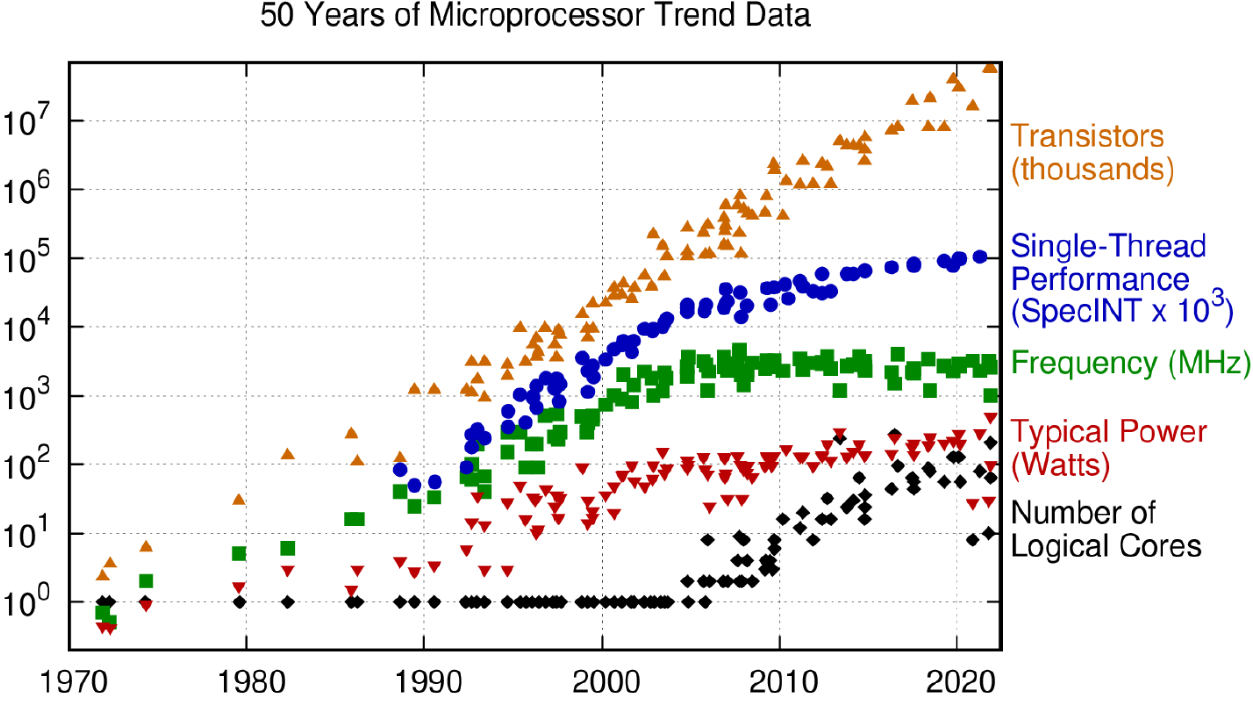
\includegraphics{images/01/cores_history.png}
   \caption{Microprocessors in the last 30 years}
   Single thread performance is increasing slowly, while the Frequency is stable.
   Moore's law is still valid if we account the number of cores.
   \label{fig:01/cores_history}
\end{figure}
{Multicore processors help reducing power for this reason:\ns
\begin{enumerate}
   \item Doubling the number of cores doubles the performance, but also power \smiley
   \item Doubling the number of cores and \textit{halving} Voltage and Frequency, leaves the same performance unaltered, but the power consumption is reduced by a factor of 4. \smiley
\end{enumerate}}

To fully exploit the potential of multicore processors, \ul{programmers need to \textbf{parallelize} our software}.
\note{There also forms of parallelization under-the-hood, which make the parallelization transparent to the developer. There also libraries that help in parallelizing the code, such as \textit{OpenMP} or \textit{FastFlow}.}

There also Heterogeneous CMPs which integrate different processor cores in a single chip, but they are more complex to handle. Common examples are the integration of a GPU in the chip, or the integration of a \textit{big.LITTLE} architecture, which integrates high-performance cores with low-power cores.
Real-world uses are some ARM processors, or the Apple M1.